\documentclass[10pt]{article}
\usepackage[a4paper,margin=17mm]{geometry}
\usepackage{mathptmx,amsmath,graphicx,booktabs,hyperref}
\setlength{\parindent}{0pt}\setlength{\parskip}{5pt}\emergencystretch=2em
\begin{document}
\begin{center}{\Large Uniform collection: unexecuted Lean source draft}\\[4pt]
Existing PR2381;26 October2026\end{center}
\textbf{No new theorem is verified.} This prepares source while checkpoint
upload authorization and token access remain pending. The file ends in
\texttt{.lean.txt}, outside all proof-gate projects. No Lean elaboration,
kernel check, axiom audit or native scientific execution occurs. Existing
208public/269audited declarations and17identities stay unchanged.

\section*{The intended bridge}
The objective remains better useful relation yield and lower relevant solver
degree for an actual twist, with a checked source-DLP reduction. The frozen
uniform protocol still plans96arms,896targets and210policy pairs on the
existing F43/F13 fixtures; no planned comparison has executed.

For coefficient space $L$, intended height is $b-\dim L$ and $N=r-1$.
List every improving successor once per query, \emph{including repeated
successors}. A stayer preserves the entire subspace, not only dimension.
The handwritten draft exposes mass conservation, positive progress,
strictly decreasing height and terminal boundary hypotheses.

\section*{Proposed algebraic statements, not checked results}
Given an explicit first-step identity with total outcome cost $c$, let
$A_F(L)$ be the sum of $F(L')$ over improving query outcomes, with repeats:
\[
 N F(L)=c+s(L)F(L)+A_F(L),
 \qquad F(L)=\frac{c+A_F(L)}{N-s(L)}.
\]
The draft targets uniqueness by decreasing height and linear scaling.
Calls use $c=N$. If $D$ is the sum of the same named query degrees at every
state, the proposed degree-request identity is $C(L)=(D/N)E(L)$.
For one remaining rank, all improving successors terminate, giving the
proposed special case $E=1/p$ with $p=(N-s)/N$.

\begin{center}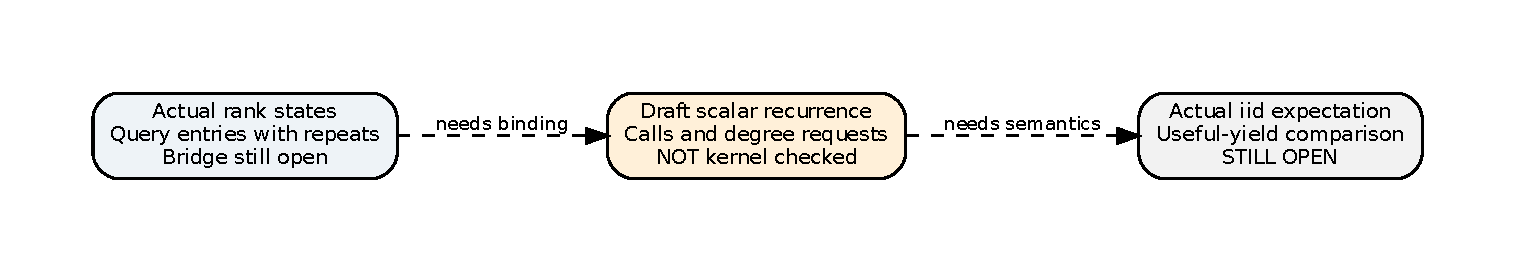
\includegraphics[width=\linewidth]{bridge.pdf}\end{center}
\textbf{What does not follow.} Larger empty-state expected rank gain alone
does not establish smaller total collection calls. The comparison draft
explicitly assumes no larger call count as well as smaller mean degree.
Degree requests are not calibrated matrix work, total DLP cost or timing.

\section*{Remaining checks and launch hold}
The first-step equation is a hypothesis, not a theorem about a random stopping
time. Actual subspace/query/source bindings, iid sampling with replacement,
absorption, integrability and probability semantics remain open. After
checkpoint-only authorization, secure token setup and successful unmodified
gate, activate a new pinned Lean project and retain all attempts through the
unmodified gate/axiom audit. Do not overwrite this draft or older proofs.
Native replay/controls and the exact experiment runner remain pending.

Source directory: \texttt{drafts/uniform-collection-20261026/}.\\
Draft file: \texttt{UniformCollection.lean.txt}.\\
Contract: \texttt{UNIFORM\_COLLECTION\_20261026\_DRAFT\_CONTRACT.md}.
Dependencies target Lean4.34.1/Mathlib\texttt{d13f23b7...}. The report uses a
diagram because no new comparable scientific values exist. No new upload,
credential reuse, paid resource, registry/benchmark row or canonical graph.
\end{document}
